\documentclass[12pt,a4paper,titlepage]{report}
\usepackage{polski}
\usepackage[utf8]{inputenc}
\usepackage{amsmath}
\usepackage{amsfonts}
\usepackage{amssymb}
\usepackage{graphicx}
\usepackage{listings}
\usepackage{enumerate}
\usepackage{color}
\definecolor{dkgreen}{rgb}{0,0.6,0}
\definecolor{gray}{rgb}{0.5,0.5,0.5}
\definecolor{mauve}{rgb}{0.58,0,0.82}
\definecolor{gray}{rgb}{0.4,0.4,0.4}
\definecolor{darkblue}{rgb}{0.0,0.0,0.6}
\definecolor{lightblue}{rgb}{0.0,0.0,0.9}
\definecolor{cyan}{rgb}{0.0,0.6,0.6}
\definecolor{darkred}{rgb}{0.6,0.0,0.0}

\author{Katarzyna Węgiełek \\ Paweł Własiuk \\ Kamil Sienkiewicz\\ Marcin Wardziński}
\title{\textbf{Computational Cluster}}
\linespread{1.125}

	
	\lstset{
  basicstyle=\ttfamily\footnotesize,
  columns=fullflexible,
  showstringspaces=false,
  numbers=left,                   % where to put the line-numbers
  numberstyle=\tiny\color{gray},  % the style that is used for the line-numbers
  stepnumber=1,
  numbersep=5pt,                  % how far the line-numbers are from the code
  backgroundcolor=\color{white},      % choose the background color. You must add \usepackage{color}
  showspaces=false,               % show spaces adding particular underscores
  showstringspaces=false,         % underline spaces within strings
  showtabs=false,                 % show tabs within strings adding particular underscores
  frame=none,                   % adds a frame around the code
  rulecolor=\color{black},        % if not set, the frame-color may be changed on line-breaks within not-black text (e.g. commens (green 	here))
  tabsize=2,                      % sets default tabsize to 2 spaces
  captionpos=b,                   % sets the caption-position to bottom
  breaklines=true,                % sets automatic line breaking
  breakatwhitespace=false,        % sets if automatic breaks should only happen at whitespace
  title=\lstname,                   % show the filename of files included with \lstinputlisting;
                                  % also try caption instead of title  
  commentstyle=\color{gray}\upshape
}
 \lstdefinelanguage{XML}
{
  morestring=[s][\color{mauve}]{"}{"},
  morestring=[s][\color{black}]{>}{<},
  morecomment=[s]{<?}{?>},
  morecomment=[s][\color{dkgreen}]{<!--}{-->},
  stringstyle=\color{black},
  identifierstyle=\color{lightblue},
  keywordstyle=\color{red},
  morekeywords={xmlns,xsi,noNamespaceSchemaLocation,type,id,x,y,source,target,version,tool,transRef,roleRef,objective,eventually},
}

\begin{document}
\maketitle
\tableofcontents

	\chapter{Wstęp}
	Tematem projektu jest stworzenie dokumentacji dla klastra obliczeniowego, który będzie umożliwiał rozwiązywanie problemów o dużej złożoności. System składa się z \textit{serwerów komunikacyjnych}, \textit{menadżerów zadań}, \textit{klientów} i \textit{węzłów obliczeniowych}.\\
Rolą \textit{serwera} jest zapewnienie komunikacji pomiędzy wszystkimi komponentami. Elementy systemu wymieniają informacje wykorzystując protokół XML. W klastrze może być kilka serwerów. Jeden z nich jest serwerem głównym - zarządza przekazywaniem komunikatów i nadzoruje stan wszystkich elementów systemu. Pozostałe pełnią rolę pomocniczą - na nich znajdują się kopie zapasowe częściowych i ostatecznych rozwiązań problemów, zadań oczekujących na rozwiązanie i informacji o trwających obliczeniach. W przypadku awarii serwera głównego, jeden z serwerów pomocniczych przejmuje jego zadania. Wykonywaniem kopii danych zajmuje się serwer główny. On też informuje menadżerów zadań, klientów oraz węzły obliczeniowe o istnieniu serwerów pomocniczych, aby w przypadku awarii możliwa była ich zamiana.\\
Zadaniem \textit{aplikacji klienckiej} jest pobranie danych wejściowych od użytkownika i wysłanie do serwera komunikacyjnego zlecenia rozwiązania podanego problemu. Gdy obliczenia zostaną zakończone, klient odbiera od serwera rozwiązanie zadania i prezentuje otrzymane wyniki użytkownikowi.\\
\textit{Menadżer zadań} zajmuje się organizacją obliczeń i uzyskaniem ostatecznego wyniku z rozwiązań cząstkowych. Po otrzymaniu problemu od serwera komunikacyjnego, dzieli go na mniejsze podproblemy, przeznaczone do rozwiązania przez pojedyncze węzły obliczeniowe. Następnie wysyła je do serwera i oczekuje na wyniki częściowe. Na ich podstawie oblicza rozwiązanie końcowe i przesyła je na serwer. Każdy menadżer zadań zawiera jeden lub kilka modułów, odpowiedzialnych za rozwiązanie konkretnego typu problemu. Wysyła on do serwera nazwy typów problemów, jakie potrafi obsłużyć, dzięki czemu serwer wie, które zadania może do niego kierować.\\
Zadaniem \textit{węzła obliczeniowego} jest rozwiązywanie podproblemów otrzymanych od serwera komunikacyjnego. Węzeł nie ma dostępu do informacji o całym zadaniu i nie zna wyników uzyskanych przez inne węzły. Otrzymuje jedynie problem częściowy, wyznaczony przez menadżera zadań, rozwiązuje go i wysyła do serwera wyniki swoich obliczeń. Węzeł składa się z jednego lub więcej modułów, zawierających algorytmy do rozwiązywania konkretnych typów podproblemów. Zanim otrzyma zadanie, wysyła do serwera informację dotyczącą rodzajów problemów, które potrafi rozwiązać. Podczas wykonywania algorytmu węzły na bieżąco informują serwer, że obliczenia trwają. W przypadku awarii węzła lub przerwania połączenia, do serwera przestaną dochodzić komunikaty i będzie on mógł skierować dany problem do innego węzła, aby uzyskać brakujący wynik częściowy.\\
Przykładowym zadaniem, które można rozwiązać korzystając z opisanego klastra obliczeniowego jest problem marszrutyzacji (Dynamic Vehicle Routing Problem).


	\chapter{Diagramy Przypadków Użycia}
		%\section{Konfiguracja}
		%	\subsection{Serwer Komunikacyjny}
		%	\subsection{Menadżer Zadań}
		%	\subsection{Węzeł obliczeniowy}
		%	\subsection{Klient}
		%\section{Komunikacja z serwerem}
		\section{Komunikacja}
			\subsection{Komponenty z serwerem}
			
			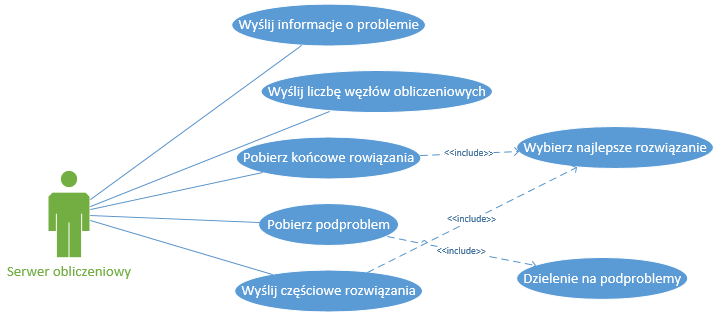
\includegraphics[width=\textwidth]{img/diagram05.png}	
			
			Cała komunikacja musi odbywać się przez serwer, dlatego na początku swojego działania każdy komponent musi się z nim połączyć. Serwer pośredniczy w przesyłaniu informacji o problemie między klientem a Menadżerem Zadań, końcowego rozwiązania od Menadżera Zadań do Klienta, jak również rozwiązań pośrednich między Węzłami Obliczeniowymi, a Menadżerem Zadań. Jego użycie jest również wymagane do przesyłania częściowych podproblemów między Menadżerem Zadań i Węzłami obliczeniowymi.
			
			Do dodatkowych funkcji serwera, nie związanych bezpośrednio z komunikacją należy podanie liczby dostępnych Węzłów obliczeniowych Menadżerowi zadań oraz informowanie o istnieniu zapasowego serwera. Serwer może zażądać informacji o klasie problemu od Menadżera Zadań i Węzłów Obliczeniowych. Węzły obliczeniowe mają obowiązek informować serwer o tym, czy obliczenia nadal się odbywają.
			\subsection{Serwer z Menadżerem Zadań}
			
			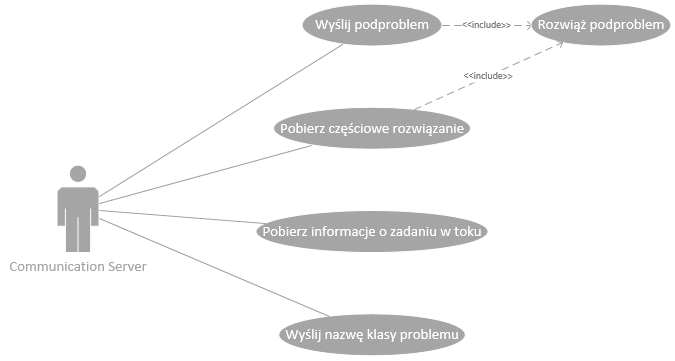
\includegraphics{img/diagram06.png}	
			
			
			\subsection{Serwer z Węzłem obliczeniowym}
			
			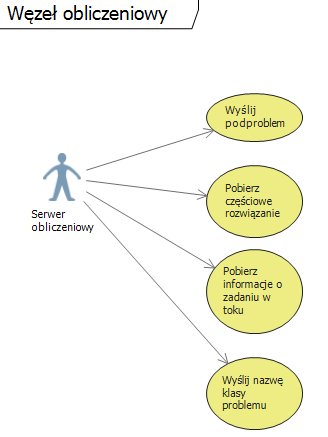
\includegraphics{img/diagram07.png}	
			
			
			\subsection{Serwer z Klientem}
			
			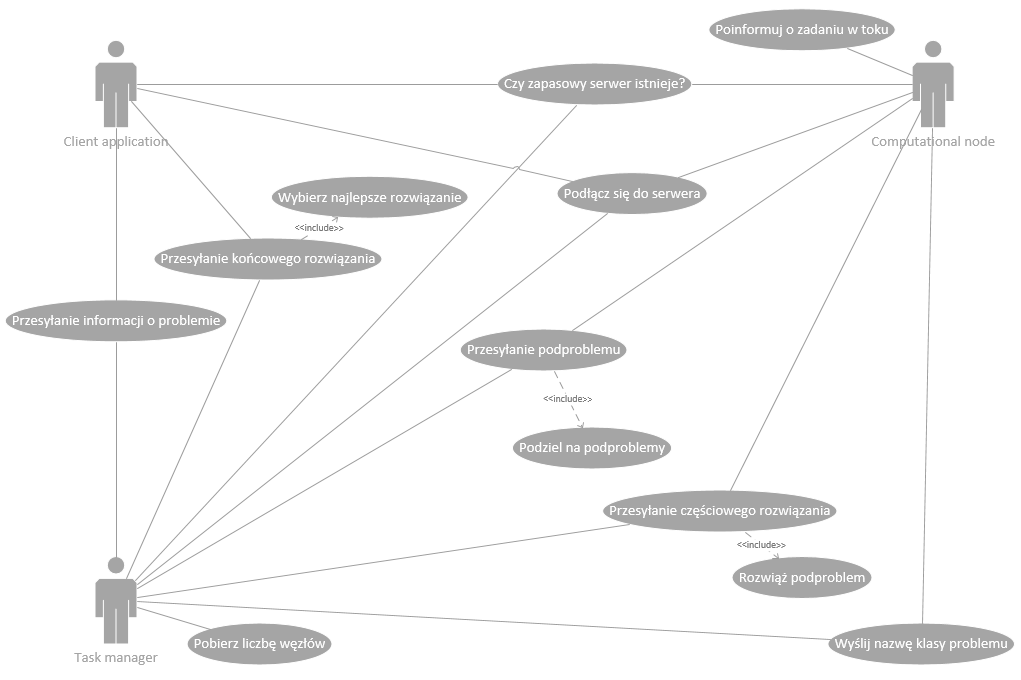
\includegraphics{img/diagram08.png}	
			
			
			
	\chapter{Diagramy Aktywności}
		\section{Zlecenie rozwiązania problemu}

		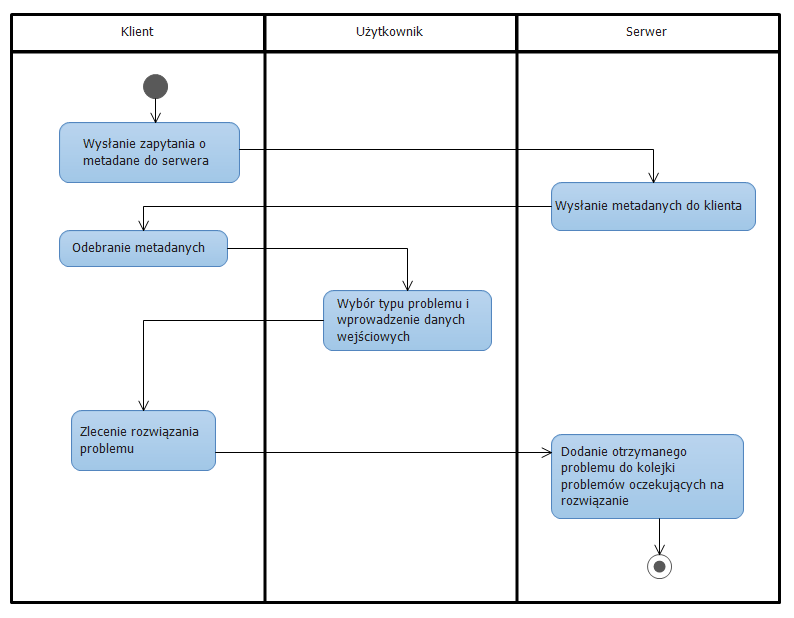
\includegraphics[width=\textwidth]{img/diagram1.png}		
		
		\textbf{Aplikacja kliencka} nawiązuje połączenie z serwerem głównym, używając adresu IP serwera zapisanego w pliku konfiguracyjnym. Wysyła zapytanie o metadane - adresy IP serwerów backup'owych oraz nazwy klas problemów, które mogą być rozwiązane przez ten klaster obliczeniowy (takie, że istnieje przynajmniej jeden \textit{menadżer zadań} potrafiący obsłużyć dany typ problemu). Serwer przesyła metadane do klienta. Następnie użytkownik wybiera spośród dostępnych nazw klas problemów typ zadania jakie ma zostać rozwiązane i wprowadza do programu wszystkie potrzebne dane wejściowe. Aplikacja kliencka wysyła do serwera zlecenie rozwiązania problemu i podane przez użytkownika dane w formacie XML.
Serwer odbiera zlecenie przysłane przez klienta i umieszcza problem w kolejce problemów danego typu oczekujących na rozwiązanie. Zadanie znajduje się w kolejce, dopóki któryś z \textit{menadżerów zadań}, potrafiących rozwiązać problem tej klasy, nie zakończy obliczeń i nie będzie mógł się nim zająć.

		\section{Odczytanie wyniku}
		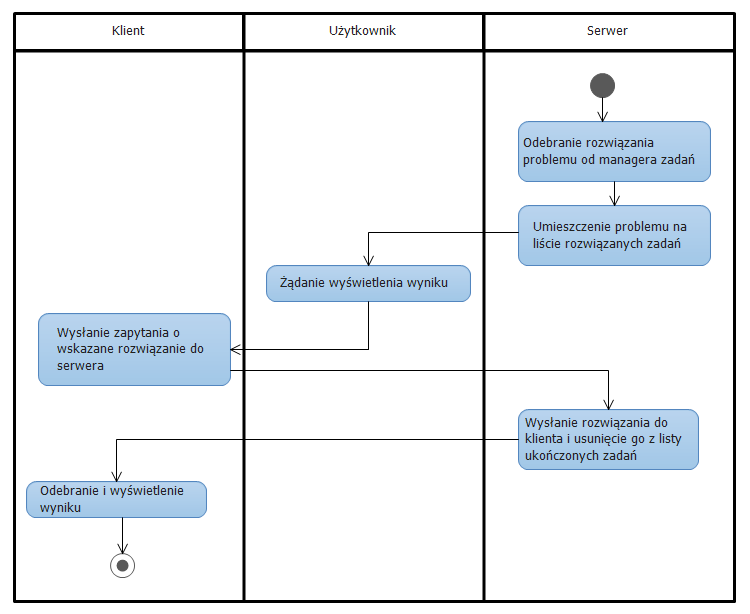
\includegraphics[width=\textwidth]{img/diagram2.png}
		Po otrzymaniu ostatecznego rozwiązania od \textit{menadżera zadań}, serwer umieszcza problem na liście ukończonych, ale jeszcze nieodczytanych rozwiązań. Następnie użytkownik wybiera z listy problem, którego rozwiązanie chce zobaczyć. Aplikacja kliencka wysyła do serwera żądanie pobrania wskazanego wyniku. Serwer wysyła rozwiązanie odpowiedniego problemu do klienta i usuwa je z listy ukończonych zadań. Klient odbiera wyniki i wyświetla je użytkownikowi.
		
		\section{Węzeł obliczeniowy}
		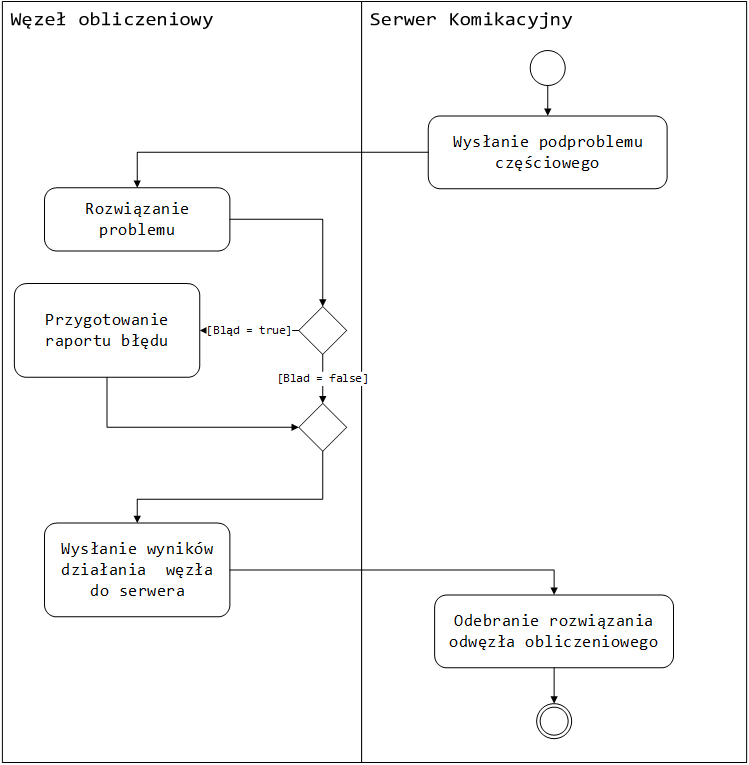
\includegraphics[width=\textwidth]{img/diagram3.png}
		Węzeł obliczeniowy przy uruchomieniu zgłasza swoją obecność serwerowi komunikacyjnemu. Informacje temat serwera 
znajdują się w pliku konfiguracyjnym węzła. Węzeł wysyła do serwera informacje na temat typów problemów które jest w stanie 
rozwiązać, dzięki temu serwer komunikacyjny może uwzględniać go przy przesyłaniu do \textbf{Menadżera Zadań} informacji na temat
ilości węzłów potrafiących rozwiązać dany typ problemu. \linebreak
Węzeł obliczeniowy nie wykonujący w danym momencie obliczeń otrzymuje od serwera skolejkowany podproblem, podzielony 
na części przez \textbf{Menadżer Zadań}. Zadaniem węzła obliczeniowego jest rozwiązanie otrzymanego zadania oraz przesłanie
rozwiązania do serwera. Jeżeli podczas wykonywania obliczeń wystąpi błąd, węzeł ma za zadanie przygotować raport o 
błędach a następnie wysłać go do serwera.

		\section{Wybieranie zadania do podzielenia}
		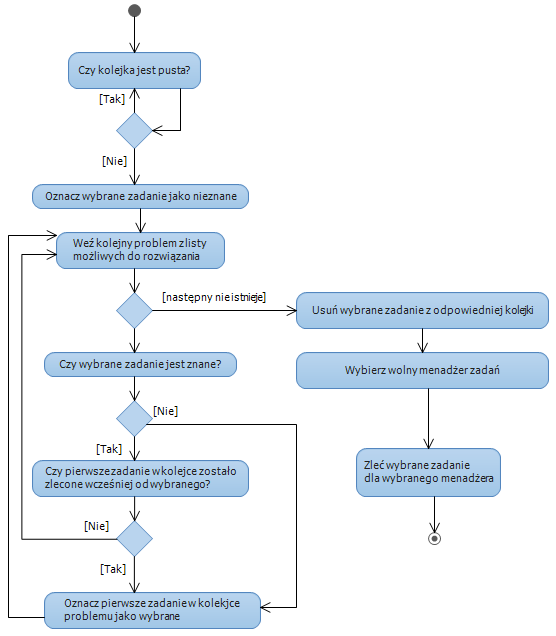
\includegraphics[width=\textwidth]{img/diagram_queue.png}
		W celu przeprowadzania procesu dzielenia problemów na podproblemy w sposób optymalny z zachowaniem kolejności
		potrzebne było opracowanie specjalnej struktury danych do ich przechowywania. (Gdzie opisać tą strukturę?
		Tutaj to się nie nadaje. Najlepiej byłoby to umieścić oddzielnie.)
		
		\section{Podział zadania na podproblemy}
		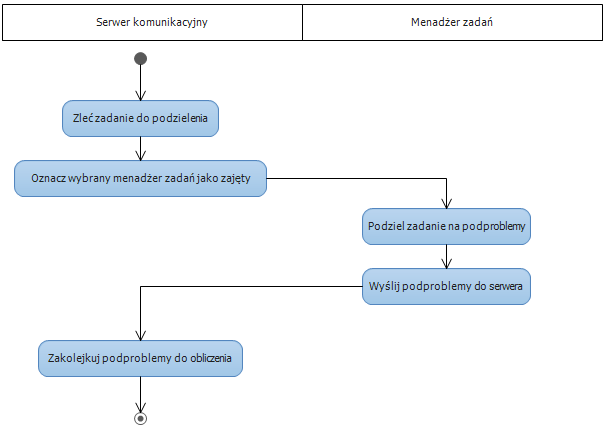
\includegraphics[width=\textwidth]{img/diagram_cstm_taskcommision.png}
		Wybrane zadanie do przetworzenia poprzez \textbf{serwer komunikacyjny} trafia do wolnego \textbf{menadżera zadań}
		potrafiącego rozwiązać dany problem. Po podzieleniu go na podproblemy, \textbf{menadżer zadań} odsyła definicje
		podproblemów z powrotem do \textbf{serwera komunikacyjnego}, który umieszcza je na innej kolejce do późniejszego
		obliczenia.
		
		\section{Zgłaszanie wyniku częściowego do menadżera zadań}
		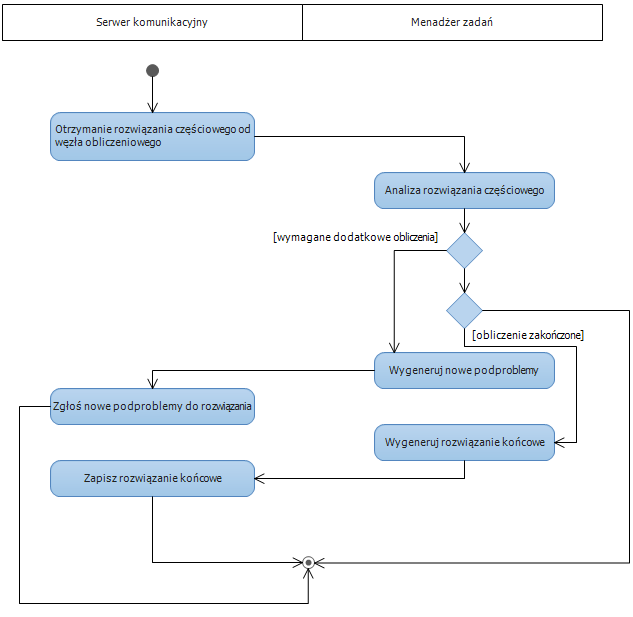
\includegraphics[width=\textwidth]{img/diagram_cstm_submitsubtasksolution.png}
		Zaraz po otrzymaniu wyniku częściowego od \textbf{węzła obliczeniowego} \textbf{serwer komunikacyjny}
		odsyła go do \textbf{menadżera zadań} który zajmuje się daną instancją problemu. \textbf{Menadżer zadań}
		po analizie rozwiązania częściowego może wygenerować nowe podproblemy, które zostaną zgłoszone analogicznie
		jak w przypadku początkowego podziału zadania. Może również oznaczyć problem jako rozwiązany i odesłać
		pełne rozwiązanie do późniejszego pobrania przez użytkownika.
		
	\chapter{Diagramy stanów}
		\section{Rodzaj zadania}
		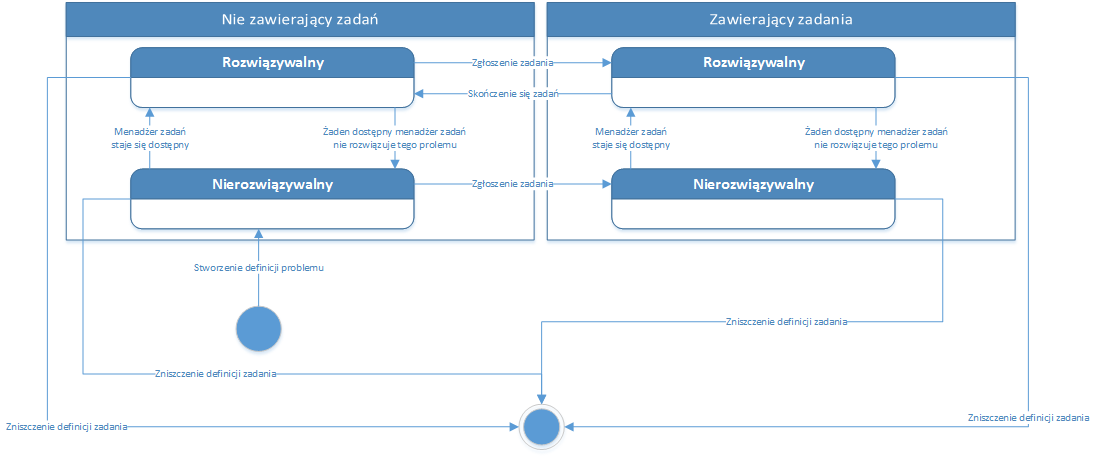
\includegraphics[width=\textwidth]{img/state/Problem.png}
		
		\section{Zadanie}
		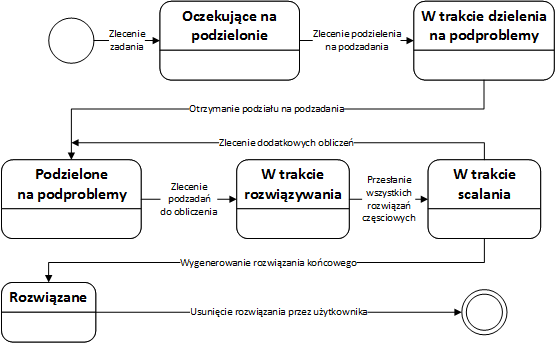
\includegraphics[width=\textwidth]{img/state/Task.png}
		
		\section{Obliczenie}
		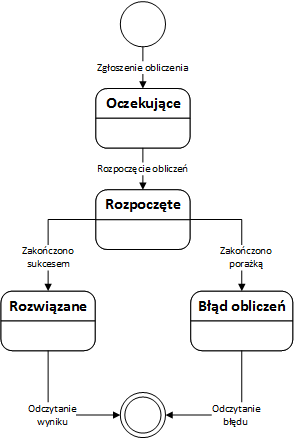
\includegraphics{img/state/Calculation.png}
		
		\section{Menadżer zadań}
		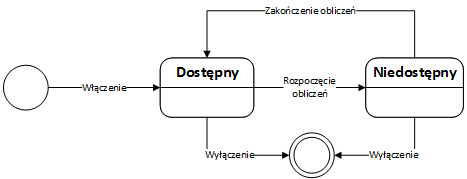
\includegraphics[width=\textwidth]{img/state/TaskManager.png}
		
		\section{Węzeł obliczeniowy}
		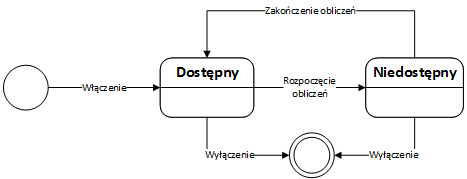
\includegraphics[width=\textwidth]{img/state/ComputationalNode.png}

	\chapter{Komunikacja}
	\section{Lista rozwiązywalnych problemów}
	Proces rozwiązywania zadania przez \textit{klaster obliczeniowy} rozpoczyna się na poziomie aplikacji klienckiej. Przed
	wysłaniem problemu do rozwiązanie, aplikacja kliencka musi pobrać z serwera informację na temat klas problemów
	rozwiązywalnych w danej chwili przez klaster obliczeniowy (wynika ona z obecnie dostępnych \textit{Menadżerów zadań} i \textit{węzłów obliczeniowych}). Aplikacja wysyła do \textit{serwera} zapytanie postaci: \\
	
	\lstinputlisting[language=XML,firstline=1,lastline=4]{examples.xml} 
	gdzie wartość węzła \verb+MessageType+ (definiującego typ wiadomości) ustawiona jest na \verb+ProblemsListRequest+.  	

	
    \textit{Serwer} w odpowiedzi na to żądanie odsyła wiadomość, w której zawarte są informacje o wszystkich typach problemów rozwiązywalnych przez klaster. Informacje zostają przetworzone i przedstawione użytkownikowi.\\
	\lstinputlisting[language=XML,firstline=7,lastline=14]{examples.xml}
	Przedstawiony powyżej fragment kodu to przykładowa odpowiedź serwera. Dla każdego typu problemu zostają przekazane dwie informacje:
	\begin{itemize}
	\item \verb+problemClassName+ - nazwa problemu,
	\item \verb+problemClassId+ - guid problemu, który w jednoznaczny sposób identyfikuje typ problemu.
	
	\end{itemize}   
	
	Ten etap komunikacji przedstawi poniższy diagram:\\
	
	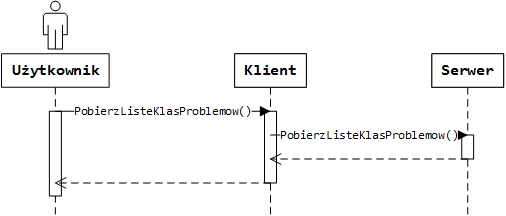
\includegraphics[width=\textwidth]{img/communication/problemclass.png}
    
    \section{Rozwiązywania zadania}
    Po wykonaniu czynności opisanych w poprzednim rozdziale, użytkownik może zlecić zadanie \textit{klastrowi obliczeniowemu}
    Aplikacja kliencka wysyła do serwera wiadomość z informacją o typie rozwiązywanego problemu, jak też danych wejściowych.
    Przykładem takiej wiadomości jest poniższy przykład: \\
    
    \lstinputlisting[language=XML,firstline=16,lastline=22]{examples.xml}
    
    Wiadomość zawiera 4 parametry konieczne do stworzenia, rozwiązania i zidentyfikowania zadania przez użytkownika:
    \begin{itemize}
    	\item \verb+MessageType+ - parametr ustawiony na \verb+TaskOrder+ informuje serwer o typie wiadomości,
    	\item \verb+problemClassId+ - identyfikator problemu, umożliwiający rozwiązanie go przed odpowiednie części systemu,
    	\item \verb+Data+ - parametry typu \verb+String+ zawierający dane wejściowe dla danego typu problemu. Dane te przedstawione są w formacie XML specyficznym dla danego typu problemu.
    	\item \verb+TaskName+ - nazwa zadania zdefiniowana przez klienta, umożliwi w przyszłości wyszukanie rozwiązania.  
    \end{itemize}
	

	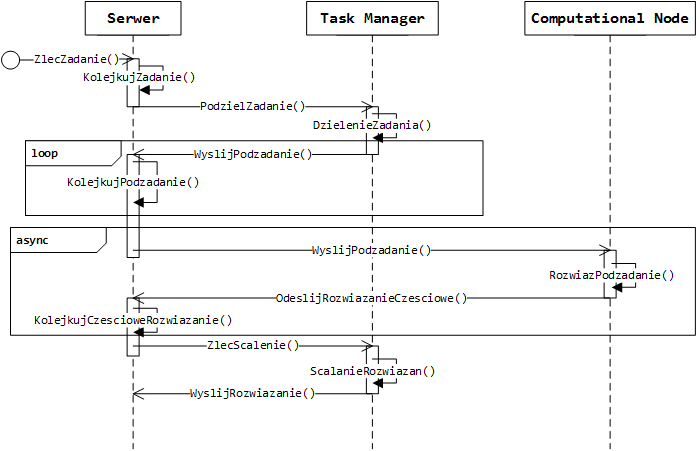
\includegraphics[width=\textwidth]{img/communication/computation.png}

	Klaster obliczeniowy wykonuje ciąg czynności koniecznych do otrzymania rozwiązania, tzn:
	\begin{enumerate}[(a)]
		\item przesłanie polecenia podziału zadania od \textit{serwera} do \textit{menadżera zadań},
		\item podział zadania i odesłanie stworzonych podproblemów prowadzących do otrzymania rozwiązania,
		\item przesłanie każdego z podzadań do \textit{węzłów obliczeniowych}
		\item przeprowadzenie obliczeń i odesłanie częściowych rozwiązań do \textit{serwera}
		\item przesłanie częsciowych rozwiązań do \textit{menadżera zadań} w celu stworzenia rozwiązania
		\item odesłanie pełnego rozwiązania zadania do \textit{serwera}
	\end{enumerate}
    
    \section{Odczytanie rozwiązania}
     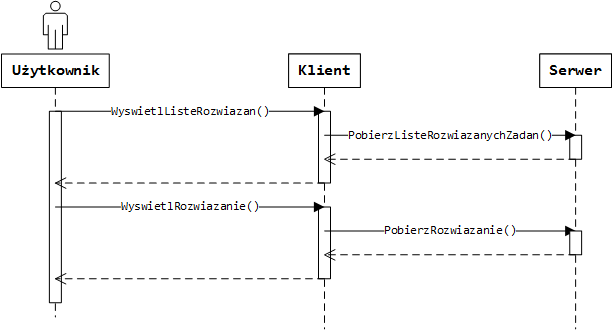
\includegraphics[width=\textwidth]{img/communication/getresult.png}
     
    Proces odczytania rozwiązania jest podobny do początkowego etapu obliczania. Tym razem \textit{aplikacja kliencka} musi poprosić \textit{serwer} o listę rozwiązanych zadań, wyświetlić je i umożliwić użytkownikowi wybór typu konkretnego zadania. 
    Razem z lista rozwiązanych problemów serwer przesyła:
    \begin{itemize}
    	\item \verb+name+ - nazwa zadania (wcześniej zdefiniowana przez użytkownika),
    	\item \verb+id+ - identyfikator zadania, wykorzystywany jest przy zapytaniu o rozwiązanie konkretnego zadania,
    	\item \verb+problemClassName+ - typ klasy problemu
    \end{itemize}
    Następnie zostaje przesłana prośba o pobranie rozwiązania dla wybranego zadania. Rozwiązanie zostaje przesłanie w postaci
    \verb+stringu+ w formacie XML specyficznym dla danego typu problemu.
    Poniżej przedstawione zostały dwa inne dwa przykłady komunikatów
    \begin{itemize}
    \item lista rozwiązanych zadań przesyłana do klienta
				\lstinputlisting[language=XML,firstline=25,lastline=32]{examples.xml}
	\item rozwiązanie przesłane do klienta
				\lstinputlisting[language=XML,firstline=35,lastline=42]{examples.xml}
   \end{itemize}
    
   
    
  

	\section{Schema}

		\lstinputlisting[language=XML]{messageSchema.xsd}
	
	
\end{document}
